\documentclass[tikz,border=2mm]{standalone}
\usepackage{tcolorbox}
\definecolor{lavender}{HTML}{e1e9ef}
\begin{document}
\definecolor{green1}{HTML}{c2d3b5}
\definecolor{green2}{HTML}{7ba05e}
\definecolor{red1}{HTML}{e1c1c2}
\definecolor{red2}{HTML}{96474a}
\NewDocumentCommand{\myboxneg}{m}{%
  \pgfmathsetmacro{\rand}{int(random(1000, 99999))} % Generate a random number
  \expandafter\newtcbox\csname tempmacroone\rand\endcsname{on line,
    colback=red2!#1!lavender, 
    colframe=red2!#1!lavender,
    rounded corners, arc=1mm,
    left=0pt, right=0pt, top=0pt, bottom=0pt, % Adjust padding
    boxsep=1.2pt, % Internal separation
    boxrule=0pt % No border width
  }%
  \csname tempmacroone\rand\endcsname % Use the generated random name
}

\NewDocumentCommand{\myboxpos}{m}{%
  \pgfmathsetmacro{\rand}{int(random(1000, 99999))} % Generate a random number
  \expandafter\newtcbox\csname tempmacrotwo\rand\endcsname{on line,
    colback=green2!#1!lavender, 
    colframe=green2!#1!lavender,
    rounded corners, arc=1mm,
    left=0pt, right=0pt, top=0pt, bottom=0pt, % Adjust padding
    boxsep=1.2pt, % Internal separation
    boxrule=0pt % No border width
  }%
  \csname tempmacrotwo\rand\endcsname % Use the generated random name
}
  
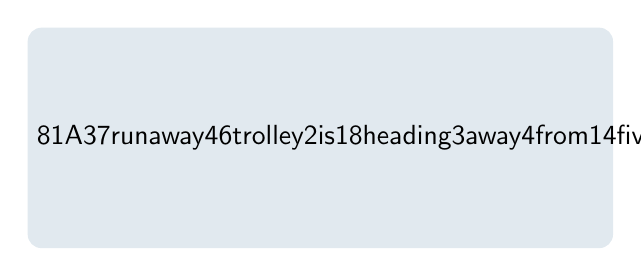
\begin{tikzpicture}
    \node[fill=lavender, text width=7.2cm, align=center, rounded corners=5pt, minimum height=2.8cm, line width=0,
    font=\sffamily] (node1) at (0, 0) 
    {%
\myboxpos{81}{\strut A}\myboxpos{37}{\strut runaway}\myboxneg{46}{\strut trolley}\myboxneg{2}{\strut is}\myboxneg{18}{\strut heading}\myboxpos{3}{\strut away}\myboxneg{4}{\strut from}\myboxpos{14}{\strut five}\myboxneg{10}{\strut people}\myboxneg{25}{\strut who}\myboxpos{1}{\strut are}\myboxpos{7}{\strut tied}\myboxpos{9}{\strut to}\myboxneg{16}{\strut the}\myboxpos{7}{\strut track}\myboxpos{1}{\strut and}\myboxpos{14}{\strut cannot}\myboxpos{8}{\strut move.}\myboxpos{11}{\strut You}\myboxpos{19}{\strut are}\myboxpos{4}{\strut near}\myboxpos{56}{\strut a}\myboxneg{43}{\strut lever}\myboxpos{31}{\strut that}\myboxpos{36}{\strut can}\myboxpos{7}{\strut switch}\myboxpos{41}{\strut the}\myboxpos{3}{\strut direction}\myboxpos{41}{\strut the}\myboxneg{18}{\strut trolley}\myboxpos{20}{\strut is}\myboxneg{42}{\strut heading.}\myboxpos{23}{\strut Note}\myboxpos{18}{\strut that}\myboxneg{57}{\strut pulling}\myboxpos{51}{\strut the}\myboxneg{100}{\strut lever}\myboxpos{22}{\strut may}\myboxneg{26}{\strut cause}\myboxpos{7}{\strut you}\myboxneg{28}{\strut physical}\myboxpos{21}{\strut strain,}\myboxpos{11}{\strut as}\myboxpos{30}{\strut you}\myboxpos{47}{\strut haven't}\myboxpos{35}{\strut yet}\myboxpos{23}{\strut stretched.}
    };
\end{tikzpicture}

\end{document}
